\documentclass[12pt]{report}
\usepackage{cleveref}
\usepackage[dutch]{babel}
\usepackage{graphicx}
\usepackage[T1]{fontenc}
\usepackage{titlesec, blindtext, color}
\definecolor{gray75}{gray}{0.75}
\newcommand{\hsp}{\hspace{20pt}}
\titleformat{\chapter}[hang]{\Huge\bfseries}{\thechapter\hsp\textcolor{gray75}{|}\hsp}{0pt}{\Huge\bfseries}
\usepackage[top=1in, bottom=1.25in, left=1.25in, right=1.25in]{geometry}



% Uncomment dit om comments te renderen in de pdf.
% http://stackoverflow.com/questions/3696128/latex-tag-for-making-a-comment-appear-or-disappear-in-pdf
% \renewenvironment{comment}{}{}

\begin{document}


\tableofcontents

\chapter{Inleiding}

Wanneer geluid wordt opgenomen is het soms handig om de opname te versnellen of te vertragen. Dit heeft tal van toepassingen, zoals bij het presenteren van het nieuws of bij het ‘beatmatchen’ van muzieknummers voor een dj. Een nieuwsanker moet veel informatie geven binnen een bepaalde tijdsspanne en af en toe gaat dit ten koste van de verstaanbaarheid. Het kan dus nuttig zijn om te snelle spraak te vertragen. Deze techniek wordt eveneens toegepast bij live muzikale optredens om op de maat te spelen.
Dit gebeurt ook wanneer het geluid bij een beeld moet gezet worden, wanneer ze niet samen zijn opgenomen. Een andere toepassing is om teksten die in een normaal tempo zijn voorgelezen te versnellen zodat blinden, die een verscherpt gehoor hebben, ook boeken kunnen 'lezen'. Het omgekeerde gebeurt voor mensen die een vreemde taal leren. [1],[2]
\cite{Thesis}
 

Als het geluid sneller of trager wordt afgespeeld door het veranderen van de bemonsteringsfrequentie, zal de toon hoger of later gaan klinken. Via \textit{time scaling} of \textit{time stretching} kan men een audiosignaal versnellen of vertragen zonder dat er een verschil in toonhoogte is. Time-scaling kan op verschillende manieren gebeuren. Algemeen worden de algoritmes opgedeeld in drie verschillende categorie\"{e}n: Time domain, Phase-vocoder en signal models. [1]. In dit verslag wordt enkel tijdsdomein algoritmes besproken, meer bepaald OLA (\textit{Overlap and Add}), SOLA (\textit{Synchronous Overlap and Add}) en PSOLA (\textit{Pitch-Synchronous Overlap and Add}). Het basisidee  van dit algoritme is eerst het splitsen in overlappende frames van het signaal en het daarna hercombineren van deze frames met telkens een bepaalde overlap om een output signaal te geven. Ten slotte worden deze algoritmes verder aangepast, zodat de time scaling ook in real time kan gebeuren.

\chapter{Time Stretching Algoritmes}
\section{Introductie}
Hoofdstuk 2 beschrijft de verschillende algoritmes voor het versnellen en vertragen van geluidsbestanden. Het hoofdstuk begint met het beschrijven van de \textit{sample rate conversion}, een slechte methode, en gaat verder met de OLA-methode (\textit{Overlap and Add}), het eenvoudigste algoritme. Vervolgens beschrijft deze tekst het SOLA-algoritme (\textit{Synchronous Overlap and Add}), wat het OLA-principe verbetert door de maximaal overeenkomende overlap te zoeken tussen de opeenvolgende frames. Een nog verbeterde versie van dit algoritme is het PSOLA (\textit{Pith-Synchronous Overlap and Add}), die gebruik maakt van de pith of toonhoogte van het signaal. Daarna wordt er een vergelijking gemaakt tussen deze algoritmes door het signaal te plotten en de frequentiespectra te vergelijking en deze te laten beoordelen in een enquete. 


\section{Sample Rate Change}
Sample rate change is een minder goede en na\"{i}eve benadering van time scaling om het geluidssignaal simpelweg te vertragen of te versnellen. Deze methode kan beschreven worden als de \textit{sample rate conversie} en versnelt of vertraagt het audiosignaal door het uit te rekken of in te krimpen over de hele lengte van het signaal. Het uitgangssignaal wordt volledig vervormd en stemmen zullen niet langer natuurlijk klinken. De voornaamste reden hiervoor is dat sample rate conversie geen rekening houdt met de verandering van de \textit{toonhoogte} of \textit{pitch}. De toonhoogte is de frequentie die het meest bepalend is voor het geluid dat de luisteraar ervaart. Zo krijg je een vervormd uitgangssignaal dat ofwel een lagere toonhoogte krijgt wanneer het fragment vertraagd wordt, ofwel een hogere toonhoogte krijgt wanneer het fragment versneld wordt.\\
\\
Sample rate conversie kan eenvoudig ge\"{i}mplementeerd worden in MATLAB door gebruik te maken van de ingebouwde functie \textit{resample}. \textbf{HIER GRAFIEKJES VAN DE OPDRACHT DIE IN DE BUNDEL STAAT OM MEE AAN TE TONEN WAAROM SAMPLE RATE CONVERSION SLECHT IS.} \\
\\\
Methodes als OLA, SOLA en PSOLA veranderen de snelheid van de geluidssignalen zonder dat informatie over de toonhoogte verloren gaat. Deze time stretching algoritmes verhinderen het negatief effect dat optreedt bij sample rate conversion en zullen een natuurlijker uitgangssignaal cre\"{e}ren.


\section{Overlap and Add (OLA)}
\subsection{Concept}
\label{subsec:OLA_concept}
Een zeer eenvoudig time stretching algoritme is het geluidssignaal te verdelen in overlappende deeltjes van een vaste lengte N. Deze originele fragmenten worden opgeschoven met een tijdsverschuiving van $ S_{a}$ samples. Vervolgens  \textbf{worden}  de blokjes gepositioneerd met een tijdsverschuiving van $S_{s}$ = $\alpha$.$S_{a}$, waarbij $\alpha$ een variabele is die vrij gekozen mag worden. De variabele $\alpha$ bepaalt in welke mate het geluidsfragment vertraagd of versneld wordt en ligt typisch tussen nul en 1/(1 - percentage overlap) omdat het outputsignaal anders gaten bevat. 

\textbf{FIGUUR MOET NOG GEHERPOSITIONEERD WORDEN}

\begin{figure}
\centering
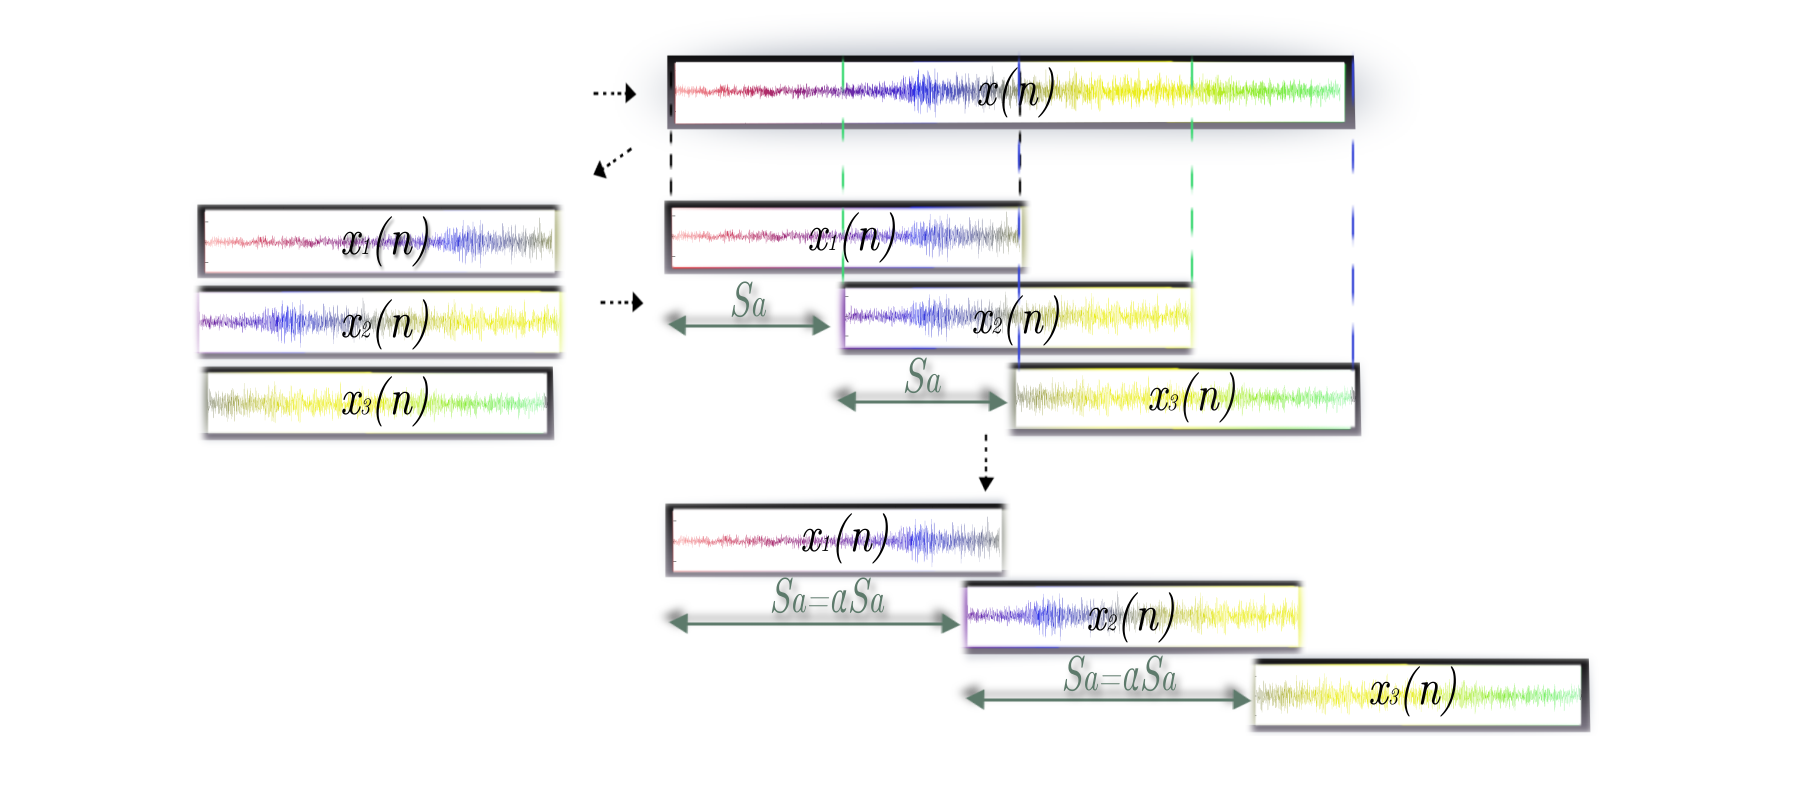
\includegraphics[width=\textwidth]{ola}
\caption{Principe van het OLA-algoritme.}
\label{fig:OLA}
\end{figure}

Door deze verschuiving overlappen kleine delen van de opeenvolgende fragmenten en op dit overlappend blok \textbf{wordt} een fade-in en fade-out functie ge\"{i}mplementeerd \textbf{(and summed sample-by-sample?)}. Uiteindelijk schakelt het algoritme de uiteengehaalde fragmenten weer aan elkaar om op deze manier een tijdsgestrekt signaal te bekomen.

\subsection{Uitwerking}
{\footnotesize \textit{\textbf{Bijlage A ???} bevat de volledige MATLAB-code voorzien van toelichting.}}\\

\noindent Deze paragraaf geeft een beschrijving van de implementatie van het OLA-algoritme in \verb+MATLAB+. De OLA-functie gebruikt vijf argumenten \cref{eq:OLA_functie}, waarvan het eerste verwijst naar het geluidssignaal dat ingeladen moet worden. Het tweede argument \verb+sample_rate+ staat voor het aantal frames per seconde waaruit het geluidssignaal bestaat en heeft een standaardwaarde van 44.100 frames/s. Het derde en laatste argument hebben dezelfde betekenis als in \cref{subsec:OLA_concept}, en hebben een defaultwaarde van respectievelijk 0,5 en 1,5. \verb+fps+ (standaard tien) verwijst naar het aantal frames per seconde en bepaalt in hoeveel frames het inputsignaal opgedeeld wordt.

\textbf{REFERENTIE WERKT NIET JUIST.}
\begin{verbatim}
\label{eq:OLA_functie}
function timeshifted_signal = timeshift_OLA(filename, sample_rate,
		                              overlap, fps, alpha)		                           
\end{verbatim}
Het OLA-algoritme bestaat uit drie grote delen. Het eerste deel laadt het audiosignaal binnen en splitst het simpelweg in twee kanalen, een linker- en een rechtersignaal. Een audiosignaal is namelijk een vector van dimensie \verb+nx2+, waarbij het aantal rijen \verb+n+ afhankelijk is van de lengte van de opname. De twee kolommen stelt het geluid voor van respectievelijk het linker- en rechtersignaal. Het programma  past verder apart de code toe op beide signalen.\\
\\
In een tweede gedeelte worden zowel het linker- als het rechtersignaal opgesplitst in frames van een vaste lengte \verb+frame_size+. De lengte \verb+frame_size+ is gelijk aan de \verb+sample_rate+ (het aantal samples per seconde) gedeeld door de \verb+fps+ (het aantal frames per seconde) en heeft als eenheid samples per frame. Het algoritme gebruikt voor het opdelen van het audiosignaal een apart geschreven functie \verb+make_frames+ (cfr. \cref{sec:bijlageA}), waarvan ook het SOLA-algoritme gebruik maakt. \\
De functie \verb+make_frames+ heeft als output een lijst \verb+frames+ waarvan elke rij de data bevat voor \'e\'en van de aparte opgesplitste fragmenten. Om deze aparte fragmenten aan te maken, hanteert de functie een \verb+for+-lus. Concreet zorgt array-slicing van het inputsignaal \textbf{(juiste terminologie?)} in elke \verb+for+-lus voor de aanmaak van een fragment.  Hierbij wordt meteen rekening gehouden met de gewilde overlap en dus zullen het begin en einde van opeenvolgende frames dezelfde data bevatten. Standaard staat de overlap op 50\%, wat inhoudt dat de tweede helft van een eerste frame volledig dezelfde data bevat als de eerste helft van het daaropvolgende frame (zie ook \cref{fig:OLA}).\\
Belangrijk is dat het algoritme bij de \verb+for+-lus het concept preallocatie toepast. Preallocatie houdt in dat \textbf{je} op voorhand de juiste lengte bepaalt van de lijst waarvan in elke \verb+for+-lus informatie wordt toegevoegd. Zo wordt tijdens elke iteratie de elementen van de lijst overschreven met deze informatie in plaats van toegevoegd zonder dat de lengte van de lijst verandert. Specifiek gaat het hier om de outputlijst \verb+frames+. Deze lijst heeft voor de lus enkel nullen, die elke iteratie overschreven worden met de data van \'e\'en afgesplitst fragment. De snelheid van het algoritme verhoogt hierdoor aanzienlijk; het duurt niet langer 15 seconden om het programma uit te voeren, maar slechts 0,3 seconden.\\
\\
Het derde en laatste deel bestaat erin om de opgesplitste fragmenten, aanwezig in de lijst \verb+frames+ (of \verb+frames_left+ en \verb+frames_right+???), te recombineren, wat resulteert in de outputlijst \verb+timeshifted_signal+ die de data voor het tijdsverschoven geluidssignaal bevat. Dit deel omvat nogmaals een \verb+for+-lus, waarbij ook hier preallocatie wordt toegepast. Concreet \textbf{worden} er tijdens elke iteratie twee indices bijgehouden, \verb+index1+ en \verb+index2+. 
\textit{ 'index1' is the index in the output signal where the overlap with the next-to-be-added frame (framel/framer) starts.
 'index2' is the index of the last sample in the output singal, where the overlap stops of course.}


\paragraph{Fade-in en fade-out:} Het algoritme werkt nu reeds "degelijk" maar een verbetering zou zijn om ...

\subsection{Interpretatie}
Het Overlap and Add principe houdt reeds een aanzienlijke verbetering in t.o.v. de ingebouwde \verb+resample+-functie van \verb+MATLAB+. Zo vertraagt en versnelt het geluidssignalen zonder de toonhoogte te veranderen, wat resulteert in een natuurlijker outputsignaal. \textbf{zie grafiek NIKKI}\\
Het bevat echt nog een aantal negatieve punten. Zo lijkt het alsof er in het uitgangssignaal enkele klanken herhaald worden. Daarnaast vertoont het signaal vrij veel ruis, zeker indien het OLA-algoritme geen crossfade functie gebruikt. Maar een groter, conceptueel probleem is dat het OLA-algoritme de informatie die aanwezig is in de data van het geluidsfragment niet benut. Het past het algoritme als het ware blind toe, wat de data ook van informatie bevat. Een beter algoritme houdt rekening met de informatie in het geluiddsignaal, zoals de locatie van de pitch.


\section{Synchronous Overlap and Add (SOLA)}
\label{sec:SOLA}

\subsection{Concept}
SOLA en OLA vertonen sterke gelijkenissen, maar het grote verschil is dat SOLA gebruikt maakt van kruiscorrelatie technieken. Dit zorgt voor minder ruis in de geluidsfragmenten.
Het algoritme verschuift de blokken met de tijdsfactor $\alpha$, en zoekt daarna naar gelijkenissen in het overlappingsgebied. Het algoritme zoekt de maximale gelijkenis en verschuift de blokken zodat deze overlappingen samenvallen. Het algoritme telt dan de uiteindelijk overlappingen weer op, zoals in het OLA-algoritme, met een crossfade. 

\subsection{Uitwerking}
De kruiscorrelatie is een manier om gelijkenissen tussen twee geluidsgolven te vinden. Het is een veelgebruikte manier bij signaalverwerking om kleinere geluidsgolven in een langer sample te herkennen, wat leidt tot patroonherkenning. Hier leidt de kruiscorrelatie tot het vinden van de index waarbij de overlapping tussen de twee frames een maximale overeenkomst vertoont.
De kruiscorrelatie wordt gegeven door :
\begin{center}
$(x_{L1}*x_{L2})[m]=\frac{1}{L} \sum\limits_{n=0}^{L-m-1}  x_{L1}^{*}[n]\cdot x_{L2}[n+m], 0 \le m < L $
\end{center}
met $x_{L1}[n]$ en $x_{L2}[n+m]$ de delen van $x_{1}[n]$ en $x_{2}[n]$ in het overlappende interval met lengte L. De index van de maximale overlap wordt gebruikt om de signalen te overlappen.
In het algoritme gebeurt de bepaling van de maximale overlapping door voor elke mogelijke overlapping een getal, de correlatie, te berekenen. Dit is de som van alle elementen in een matrix, gedeeld door de lengte van de overlapping. De matrix is gelijk aan de element-per-element vermenigvuldiging van het eerste deeltje en het tweede overlappende deel. In de code staat dit als:
\textbf{FIGUUR MOET NOG GEHERPOSITIONEERD WORDEN}
\begin{figure}
\centering
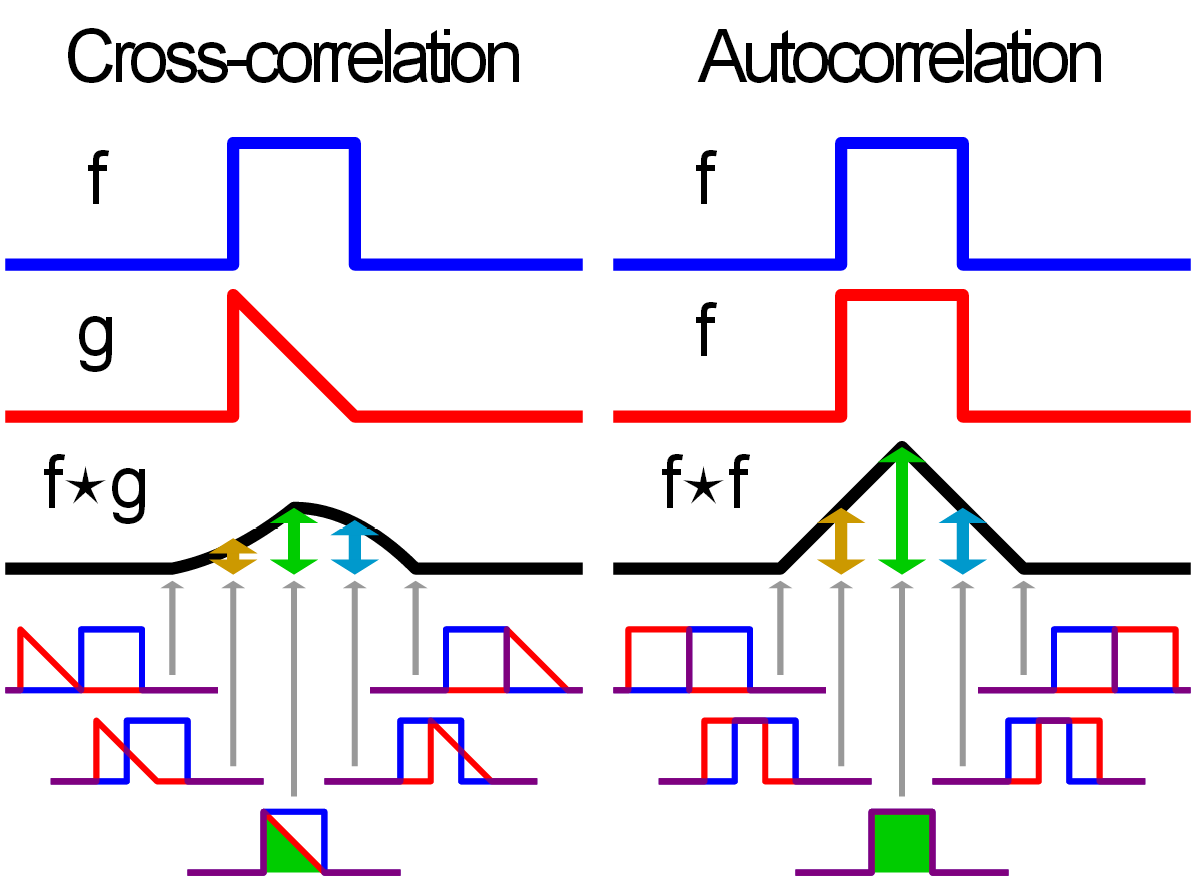
\includegraphics[width=\textwidth]{crossautocorrelatie}
\caption{Principe van cross- en autocorrelatie.}
\label{fig:crosscorrelatie}
\end{figure}



\begin{verbatim}
$correlation = sum(overlapping_part_of_output_signal .* ...
overlapping_part_of_frame) / length_overlap;
\end{verbatim}

Als dit getal groter is dan \verb|max_correlation|, de maximale waarde tot nu toe  vervangen door de nieuwe maximale waarde, dan wordt de corresponderende \verb|max_correlation_index| ook vervangen.
Zo wordt de grootste waarde voor de kruiscorrelatie bepaald, alsook op welke positie van overlapping dit gebeurd. De twee delen worden dan zo verschuiven zodat het tweede stukje begint op de index van \verb|max_correlation_index|. De frames worden opgeteld met een kruisfade en dit wordt herhaald voor alle frames. Dit wordt ook grafisch weergegeven in \textbf{grafiek???}

\section{Pitch-Synchronous Overlap and Add (PSOLA)}
Pitch-Synchronous Overlap Add maakt gebruik van de veronderstelling dat geluid gekenmerkt is door zijn toonhoogte. Het synchroniseert kleine overlappende geluidsfragmenten op basis van deze toonhoogtes om zo discontinuïteiten te voorkomen. 
Allereerst detecteert het algoritme periodisch de toonhoogte van elk geluidsframe waarin het geheel wordt opgedeeld en houdt de plaats ervan bij in de tijd (pitch mark). Door gebruik te maken van een Hanning-venster wordt het geluidsfragment rond elke pitch mark apart geëxtraheerd. De lengte van het Hanning-venster is gelijk aan het dubbele van de periode zodat later de fade-in en fade-out correct werkt.
Vervolgens voegt het algoritme de frames samen via volgend principe: afhankelijk van de variabele alpha (die de versnelling of vertraging bepaald) wordt als volgend geluidsframe dat frame genomen waarvan de pitch mark het dichtstbij ligt. Zo kan het dus dat frames worden overgeslagen of dubbel genomen. Na het overlappen en optellen van de frames kijkt het algoritme naar de volgende pitch mark en herhaalt de bovenbeschreven stappen.


\section{Pitch Detection} 

\subsection{concept}

De toonhoogte('pitch') is een attribuut dat wordt geassocieerd met de geluidsfrequentie. Afhankelijk van de frequentie van het signaal, wordt er een bepaalde toonhoogte aan gegeven. Ondanks het feit dat de twee niet equivalent zijn, zal de informatie afkomstig van de toonhoogte een kritieke rol spelen bij het 
verbeteren van de voordien besproken time-stretching algoritmes.

\subsection{Zero-crossing rate}

De zero-crossing rate is een elementair 'pitch-detection' algoritme. Het werkt goed in de afwezigheid van ruis en wordt hier besproken vanwege zijn simpelheid en rekentijd. De zero-crossing rate bepaalt hoeveel keer de geluidsgolf de x-as snijdt in een bepaald tijdsinterval.

\subsubsection{uitwerking}

We definiëren een sign {} dat een +1 of 0 teruggeeft afhankelijk van het feit dat het signaal 0 is of niet. De zero-crossing rate (ZCR) mag gezien worden als:
\begin{center}
$ZCR=\frac{1}{N} \sum\limits_{n=0}^{N-1} |sign\{s(n)-sign\{s(n-1)\}\}|$
\end{center}

\subsection{Pitch detectie met auto-correlatie}
Een meer robuuste manier om pitch detectie uit te voeren is door gebruik te maken van de autocorrelatie van een signaal. De autocorrelatie is gelijkend op de kruiscorrelatie in (?? verwijzing), maar bij de autocorrelatie wordt het algoritme toegepast op hetzelfde signaal. 
Een venster van twee maal de lengte van de langste periode wordt  gebruikt om accuraat de pitch te bepalen. Als de shift in de auto-correlatie functie de fundamentele frequentie, bereikt de autocorrelatie een maximum. Dit maximum kan beschouwd worden als de pitch periode. Zo is het mogelijk om de pitch periode te bepalen van het signaal. 

%Code bekijken en verder aanvullen

%Vergelijking moet nog uitgeschreven worden 
\section{Vergelijking verschillende algoritmes}
\subsection{Frequentie en signaal plots}
\subsection{Enquete}



\chapter{Real-time implementatie}
In het implementeren van de voorgaande algoritmes werd steeds gebruikt gemaakt van reeds opgenomen signalen, waarvan de karakteristieken gekend waren. In real-time-implementatie zijn de signaal karakteristieken ongekend en veranderen ze doorheen de tijd. Het signaal kan niet versneld worden omdat er niet in de toekomst kan gekeken worden en de daarna komende frames niet gekend zijn. Het signaal vertragen kan echter wel, omdat er stukjes van het gekende signaal moeten herhaald worden. Dit is de volgende stap die nog verder uitgewerkt moet worden in de volgende teamzittingen. Dit zal gebeuren in simulink. Wanneer het algoritme in simulink werkt, wordt het samengevoegd met de wim de vilder filter, die gemaakt werd door een ander team, om de ademhalingsruis eruit te halen.

\chapter{Werkwijze en vakintegratie}
\section{Werkwijze}
Elke P\&O zitting begint met een korte vergadering. Hierin bespreken we eerst de eventuele huistaken en hoe deze verlopen zijn. Dan passen we indien nodig de  algemene planning aan en stellen we de dagplanning op met de taakverdeling. Dit gebeurt in Asana, een handige webinterface diealle projecttaken makkelijk laat inplannen. Vervolgens maken we via Instagantt een Gant-chart voor een duidelijk overzicht. 
Als er moet geprogrammeerd worden proberen we in groepjes van twee te werken. Volgens het ‘Pair Programming’-systeem kan dan één persoon de code typen en de andere kijkt onmiddellijk na op fouten. 
\section{Vakintegratie}

Bij dit project wordt de kennis uit verschillende vakken toegepast. Het project werkt met geluid. Een matrix stelt het geluid voor. Bewerkingen op matrices werd aangeleerd in het vak toegpaste algebra. Het frequentiespectrum kan berekend worden door een fourier transformatie. Dit werd gezien in het vak Informatie-Overdracht en Verwerking en in Elektrische Netwerken. Het schrijven van de algoritmes in Matlab vergt kennis opgedaan uit het vak methodiek van de informatica. In de algoritmes wordt ook gebruikt gemaakt van een crosscorrelatie die werkt met een convolutie. Dit staat uitgelegd in de cursus Algebra en Analyse. Daarnaast wordt de kennis van PenO 1 en 2 toegepast in de vergaderingen. 
>>>>>>> lay out verslag aangepast en references.bib toegevoegd

\chapter{Besluit}







\chapter{Bijlages}
\section{Bijlage A}
\label{sec:bijlageA}

\section{Bijlage B}


\bibliographystyle{plain}
\bibliography{references}

\chapter{Tijdelijke Commentaar}

\section{Informele inhoudstafel}
Wat moet er zeker in het verslag?
\begin{enumerate}
\item Inleiding
\begin{itemize}
\item Situering van het probleem in context
\item (Verband met literatuur/evt. vorige studies)
\item Heel kort opsommen van voornaamste besluiten
\item Structuur/opbouw van het verslag duiden
\end{itemize}
\item Middenstuk
\begin{itemize}
\item Sample Rate change
\item Time Stretching Algorithms: OLA, SOLA, PSOLA, Pitch Detection
\begin{enumerate}
\item \textbf{Concept:} uitleg algemeen principe (conceptueel schetsen)
\item \textbf{Uitwerking:} code in MATLAB + duiding (specifieke uitleg)
\item \textbf{Interpretatie:} reflectie/interpretatie/besluit: is dit een goed algoritme of niet? Waarom wel/niet? Wat kan beter?
\end{enumerate}
\item Real-time implementatie/Simulink
\end{itemize}
\item Slot
\begin{itemize}
\item Integratie andere vakken
\item Reflectie planning
\item Conclusie
\end{itemize}
\item Referentielijst
\item Bijlages
\end{enumerate}

\section{Algemene opmerkingen}
\begin{itemize}
\item Chapters vernederlandsen
\item Cross-referenties goed krijgen
\item Formule crosscorelatie
\item Foto crosscorelatie
\item Foto's invoegen
\item titels terug toevoegen?
\item interpretatie?
\item Foto's op de juiste plaats zien te krijgen.
\item zien wat er niet mee upgedatet is.
\item zien dat de indent bij elke paragraaf consistent is.

\end{itemize}





\end{document}
